\documentclass[1p]{elsarticle_modified}
%\bibliographystyle{elsarticle-num}

%\usepackage[colorlinks]{hyperref}
%\usepackage{abbrmath_seonhwa} %\Abb, \Ascr, \Acal ,\Abf, \Afrak
\usepackage{amsfonts}
\usepackage{amssymb}
\usepackage{amsmath}
\usepackage{amsthm}
\usepackage{scalefnt}
\usepackage{amsbsy}
\usepackage{kotex}
\usepackage{caption}
\usepackage{subfig}
\usepackage{color}
\usepackage{graphicx}
\usepackage{xcolor} %% white, black, red, green, blue, cyan, magenta, yellow
\usepackage{float}
\usepackage{setspace}
\usepackage{hyperref}

\usepackage{tikz}
\usetikzlibrary{arrows}

\usepackage{multirow}
\usepackage{array} % fixed length table
\usepackage{hhline}

%%%%%%%%%%%%%%%%%%%%%
\makeatletter
\renewcommand*\env@matrix[1][\arraystretch]{%
	\edef\arraystretch{#1}%
	\hskip -\arraycolsep
	\let\@ifnextchar\new@ifnextchar
	\array{*\c@MaxMatrixCols c}}
\makeatother %https://tex.stackexchange.com/questions/14071/how-can-i-increase-the-line-spacing-in-a-matrix
%%%%%%%%%%%%%%%

\usepackage[normalem]{ulem}

\newcommand{\msout}[1]{\ifmmode\text{\sout{\ensuremath{#1}}}\else\sout{#1}\fi}
%SOURCE: \msout is \stkout macro in https://tex.stackexchange.com/questions/20609/strikeout-in-math-mode

\newcommand{\cancel}[1]{
	\ifmmode
	{\color{red}\msout{#1}}
	\else
	{\color{red}\sout{#1}}
	\fi
}

\newcommand{\add}[1]{
	{\color{blue}\uwave{#1}}
}

\newcommand{\replace}[2]{
	\ifmmode
	{\color{red}\msout{#1}}{\color{blue}\uwave{#2}}
	\else
	{\color{red}\sout{#1}}{\color{blue}\uwave{#2}}
	\fi
}

\newcommand{\Sol}{\mathcal{S}} %segment
\newcommand{\D}{D} %diagram
\newcommand{\A}{\mathcal{A}} %arc


%%%%%%%%%%%%%%%%%%%%%%%%%%%%%5 test

\def\sl{\operatorname{\textup{SL}}(2,\Cbb)}
\def\psl{\operatorname{\textup{PSL}}(2,\Cbb)}
\def\quan{\mkern 1mu \triangleright \mkern 1mu}

\theoremstyle{definition}
\newtheorem{thm}{Theorem}[section]
\newtheorem{prop}[thm]{Proposition}
\newtheorem{lem}[thm]{Lemma}
\newtheorem{ques}[thm]{Question}
\newtheorem{cor}[thm]{Corollary}
\newtheorem{defn}[thm]{Definition}
\newtheorem{exam}[thm]{Example}
\newtheorem{rmk}[thm]{Remark}
\newtheorem{alg}[thm]{Algorithm}

\newcommand{\I}{\sqrt{-1}}
\begin{document}

%\begin{frontmatter}
%
%\title{Boundary parabolic representations of knots up to 8 crossings}
%
%%% Group authors per affiliation:
%\author{Yunhi Cho} 
%\address{Department of Mathematics, University of Seoul, Seoul, Korea}
%\ead{yhcho@uos.ac.kr}
%
%
%\author{Seonhwa Kim} %\fnref{s_kim}}
%\address{Center for Geometry and Physics, Institute for Basic Science, Pohang, 37673, Korea}
%\ead{ryeona17@ibs.re.kr}
%
%\author{Hyuk Kim}
%\address{Department of Mathematical Sciences, Seoul National University, Seoul 08826, Korea}
%\ead{hyukkim@snu.ac.kr}
%
%\author{Seokbeom Yoon}
%\address{Department of Mathematical Sciences, Seoul National University, Seoul, 08826,  Korea}
%\ead{sbyoon15@snu.ac.kr}
%
%\begin{abstract}
%We find all boundary parabolic representation of knots up to 8 crossings.
%
%\end{abstract}
%\begin{keyword}
%    \MSC[2010] 57M25 
%\end{keyword}
%
%\end{frontmatter}

%\linenumbers
%\tableofcontents
%
\newcommand\colored[1]{\textcolor{white}{\rule[-0.35ex]{0.8em}{1.4ex}}\kern-0.8em\color{red} #1}%
%\newcommand\colored[1]{\textcolor{white}{ #1}\kern-2.17ex	\textcolor{white}{ #1}\kern-1.81ex	\textcolor{white}{ #1}\kern-2.15ex\color{red}#1	}

{\Large $\underline{12n_{0772}~(K12n_{0772})}$}

\setlength{\tabcolsep}{10pt}
\renewcommand{\arraystretch}{1.6}
\vspace{1cm}\begin{tabular}{m{100pt}>{\centering\arraybackslash}m{274pt}}
\multirow{5}{120pt}{
	\centering
	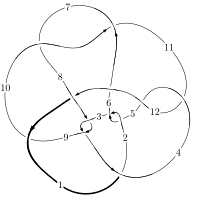
\includegraphics[width=112pt]{../../../GIT/diagram.site/Diagrams/png/2861_12n_0772.png}\\
\ \ \ A knot diagram\footnotemark}&
\allowdisplaybreaks
\textbf{Linearized knot diagam} \\
\cline{2-2}
 &
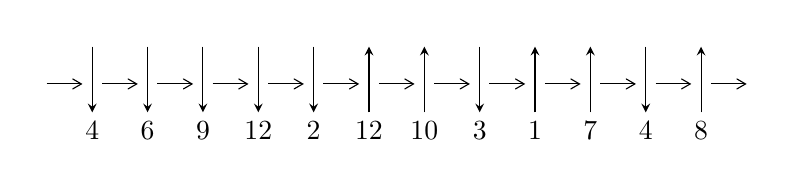
\begin{tikzpicture}[x=20pt, y=17pt]
	% nodes
	\node (C0) at (0, 0) {};
	\node (C1) at (1, 0) {};
	\node (C1U) at (1, +1) {};
	\node (C1D) at (1, -1) {4};

	\node (C2) at (2, 0) {};
	\node (C2U) at (2, +1) {};
	\node (C2D) at (2, -1) {6};

	\node (C3) at (3, 0) {};
	\node (C3U) at (3, +1) {};
	\node (C3D) at (3, -1) {9};

	\node (C4) at (4, 0) {};
	\node (C4U) at (4, +1) {};
	\node (C4D) at (4, -1) {12};

	\node (C5) at (5, 0) {};
	\node (C5U) at (5, +1) {};
	\node (C5D) at (5, -1) {2};

	\node (C6) at (6, 0) {};
	\node (C6U) at (6, +1) {};
	\node (C6D) at (6, -1) {12};

	\node (C7) at (7, 0) {};
	\node (C7U) at (7, +1) {};
	\node (C7D) at (7, -1) {10};

	\node (C8) at (8, 0) {};
	\node (C8U) at (8, +1) {};
	\node (C8D) at (8, -1) {3};

	\node (C9) at (9, 0) {};
	\node (C9U) at (9, +1) {};
	\node (C9D) at (9, -1) {1};

	\node (C10) at (10, 0) {};
	\node (C10U) at (10, +1) {};
	\node (C10D) at (10, -1) {7};

	\node (C11) at (11, 0) {};
	\node (C11U) at (11, +1) {};
	\node (C11D) at (11, -1) {4};

	\node (C12) at (12, 0) {};
	\node (C12U) at (12, +1) {};
	\node (C12D) at (12, -1) {8};
	\node (C13) at (13, 0) {};

	% arrows
	\draw[->,>={angle 60}]
	(C0) edge (C1) (C1) edge (C2) (C2) edge (C3) (C3) edge (C4) (C4) edge (C5) (C5) edge (C6) (C6) edge (C7) (C7) edge (C8) (C8) edge (C9) (C9) edge (C10) (C10) edge (C11) (C11) edge (C12) (C12) edge (C13) ;	\draw[->,>=stealth]
	(C1U) edge (C1D) (C2U) edge (C2D) (C3U) edge (C3D) (C4U) edge (C4D) (C5U) edge (C5D) (C6D) edge (C6U) (C7D) edge (C7U) (C8U) edge (C8D) (C9D) edge (C9U) (C10D) edge (C10U) (C11U) edge (C11D) (C12D) edge (C12U) ;
	\end{tikzpicture} \\
\hhline{~~} \\& 
\textbf{Solving Sequence} \\ \cline{2-2} 
 &
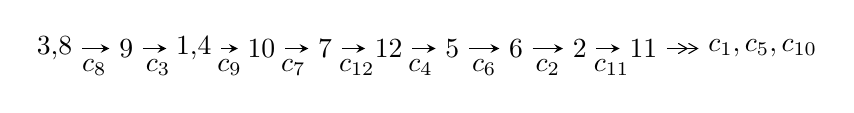
\begin{tikzpicture}[x=23pt, y=7pt]
	% node
	\node (A0) at (-1/8, 0) {3,8};
	\node (A1) at (1, 0) {9};
	\node (A2) at (33/16, 0) {1,4};
	\node (A3) at (25/8, 0) {10};
	\node (A4) at (33/8, 0) {7};
	\node (A5) at (41/8, 0) {12};
	\node (A6) at (49/8, 0) {5};
	\node (A7) at (57/8, 0) {6};
	\node (A8) at (65/8, 0) {2};
	\node (A9) at (73/8, 0) {11};
	\node (C1) at (1/2, -1) {$c_{8}$};
	\node (C2) at (3/2, -1) {$c_{3}$};
	\node (C3) at (21/8, -1) {$c_{9}$};
	\node (C4) at (29/8, -1) {$c_{7}$};
	\node (C5) at (37/8, -1) {$c_{12}$};
	\node (C6) at (45/8, -1) {$c_{4}$};
	\node (C7) at (53/8, -1) {$c_{6}$};
	\node (C8) at (61/8, -1) {$c_{2}$};
	\node (C9) at (69/8, -1) {$c_{11}$};
	\node (A10) at (11, 0) {$c_{1},c_{5},c_{10}$};

	% edge
	\draw[->,>=stealth]	
	(A0) edge (A1) (A1) edge (A2) (A2) edge (A3) (A3) edge (A4) (A4) edge (A5) (A5) edge (A6) (A6) edge (A7) (A7) edge (A8) (A8) edge (A9) ;
	\draw[->>,>={angle 60}]	
	(A9) edge (A10);
\end{tikzpicture} \\ 

\end{tabular} \\

\footnotetext{
The image of knot diagram is generated by the software ``\textbf{Draw programme}" developed by Andrew Bartholomew(\url{http://www.layer8.co.uk/maths/draw/index.htm\#Running-draw}), where we modified some parts for our purpose(\url{https://github.com/CATsTAILs/LinksPainter}).
}\phantom \\ \newline 
\centering \textbf{Ideals for irreducible components\footnotemark of $X_{\text{par}}$} 
 
\begin{align*}
I^u_{1}&=\langle 
-2.73255\times10^{170} u^{87}+3.77083\times10^{170} u^{86}+\cdots+1.71978\times10^{169} b+4.69942\times10^{170},\\
\phantom{I^u_{1}}&\phantom{= \langle  }-7.39052\times10^{170} u^{87}+1.04203\times10^{171} u^{86}+\cdots+1.71978\times10^{169} a+1.27642\times10^{171},\\
\phantom{I^u_{1}}&\phantom{= \langle  }u^{88}-2 u^{87}+\cdots-7 u^2+1\rangle \\
I^u_{2}&=\langle 
1869070191 u^{24}+1444290010 u^{23}+\cdots+1044856181 b+1214090807,\\
\phantom{I^u_{2}}&\phantom{= \langle  }7580555710 u^{24}+8345483601 u^{23}+\cdots+1044856181 a-1136568902,\;u^{25}+u^{24}+\cdots-9 u^2+1\rangle \\
\\
\end{align*}
\raggedright * 2 irreducible components of $\dim_{\mathbb{C}}=0$, with total 113 representations.\\
\footnotetext{All coefficients of polynomials are rational numbers. But the coefficients are sometimes approximated in decimal forms when there is not enough margin.}
\newpage
\renewcommand{\arraystretch}{1}
\centering \section*{I. $I^u_{1}= \langle -2.73\times10^{170} u^{87}+3.77\times10^{170} u^{86}+\cdots+1.72\times10^{169} b+4.70\times10^{170},\;-7.39\times10^{170} u^{87}+1.04\times10^{171} u^{86}+\cdots+1.72\times10^{169} a+1.28\times10^{171},\;u^{88}-2 u^{87}+\cdots-7 u^2+1 \rangle$}
\flushleft \textbf{(i) Arc colorings}\\
\begin{tabular}{m{7pt} m{180pt} m{7pt} m{180pt} }
\flushright $a_{3}=$&$\begin{pmatrix}0\\u\end{pmatrix}$ \\
\flushright $a_{8}=$&$\begin{pmatrix}1\\0\end{pmatrix}$ \\
\flushright $a_{9}=$&$\begin{pmatrix}1\\u^2\end{pmatrix}$ \\
\flushright $a_{1}=$&$\begin{pmatrix}42.9735 u^{87}-60.5909 u^{86}+\cdots-109.824 u-74.2200\\15.8889 u^{87}-21.9262 u^{86}+\cdots-39.2450 u-27.3257\end{pmatrix}$ \\
\flushright $a_{4}=$&$\begin{pmatrix}- u\\- u^3+u\end{pmatrix}$ \\
\flushright $a_{10}=$&$\begin{pmatrix}-29.6028 u^{87}+33.5360 u^{86}+\cdots+25.1212 u+32.7939\\7.55835 u^{87}-9.72166 u^{86}+\cdots-17.3864 u-11.9790\end{pmatrix}$ \\
\flushright $a_{7}=$&$\begin{pmatrix}20.5958 u^{87}-33.3831 u^{86}+\cdots-72.8706 u-43.0649\\5.79378 u^{87}-7.20014 u^{86}+\cdots-11.8431 u-9.92354\end{pmatrix}$ \\
\flushright $a_{12}=$&$\begin{pmatrix}27.0846 u^{87}-38.6647 u^{86}+\cdots-70.5794 u-46.8944\\15.8889 u^{87}-21.9262 u^{86}+\cdots-39.2450 u-27.3257\end{pmatrix}$ \\
\flushright $a_{5}=$&$\begin{pmatrix}6.81156 u^{87}-7.84254 u^{86}+\cdots-10.9251 u-11.1767\\-10.4758 u^{87}+9.82933 u^{86}+\cdots+5.39362 u+10.8270\end{pmatrix}$ \\
\flushright $a_{6}=$&$\begin{pmatrix}-20.5261 u^{87}+28.6221 u^{86}+\cdots+55.1947 u+37.5188\\-16.5192 u^{87}+24.9588 u^{86}+\cdots+53.4694 u+32.4270\end{pmatrix}$ \\
\flushright $a_{2}=$&$\begin{pmatrix}26.3861 u^{87}-36.7076 u^{86}+\cdots-64.1178 u-45.1799\\27.6983 u^{87}-38.1481 u^{86}+\cdots-68.3642 u-47.0744\end{pmatrix}$ \\
\flushright $a_{11}=$&$\begin{pmatrix}39.6126 u^{87}-56.9442 u^{86}+\cdots-105.928 u-69.0794\\6.68892 u^{87}-9.17729 u^{86}+\cdots-16.4241 u-11.9172\end{pmatrix}$\\&\end{tabular}
\flushleft \textbf{(ii) Obstruction class $= -1$}\\~\\
\flushleft \textbf{(iii) Cusp Shapes $= -19.2430 u^{87}+15.1487 u^{86}+\cdots-24.6831 u+10.9472$}\\~\\
\newpage\renewcommand{\arraystretch}{1}
\flushleft \textbf{(iv) u-Polynomials at the component}\newline \\
\begin{tabular}{m{50pt}|m{274pt}}
Crossings & \hspace{64pt}u-Polynomials at each crossing \\
\hline $$\begin{aligned}c_{1}\end{aligned}$$&$\begin{aligned}
&u^{88}+8 u^{86}+\cdots-22991 u-4937
\end{aligned}$\\
\hline $$\begin{aligned}c_{2},c_{5}\end{aligned}$$&$\begin{aligned}
&u^{88}+4 u^{87}+\cdots+5 u-79
\end{aligned}$\\
\hline $$\begin{aligned}c_{3},c_{8}\end{aligned}$$&$\begin{aligned}
&u^{88}+2 u^{87}+\cdots-7 u^2+1
\end{aligned}$\\
\hline $$\begin{aligned}c_{4},c_{11}\end{aligned}$$&$\begin{aligned}
&u^{88}+u^{87}+\cdots+43878 u-1549
\end{aligned}$\\
\hline $$\begin{aligned}c_{6}\end{aligned}$$&$\begin{aligned}
&u^{88}-2 u^{87}+\cdots+2779127 u-52466021
\end{aligned}$\\
\hline $$\begin{aligned}c_{7},c_{10}\end{aligned}$$&$\begin{aligned}
&u^{88}+5 u^{87}+\cdots-39868 u-4364
\end{aligned}$\\
\hline $$\begin{aligned}c_{9}\end{aligned}$$&$\begin{aligned}
&u^{88}-6 u^{87}+\cdots-2747 u-199
\end{aligned}$\\
\hline $$\begin{aligned}c_{12}\end{aligned}$$&$\begin{aligned}
&u^{88}+2 u^{87}+\cdots+4454 u-497
\end{aligned}$\\
\hline
\end{tabular}\\~\\
\newpage\renewcommand{\arraystretch}{1}
\flushleft \textbf{(v) Riley Polynomials at the component}\newline \\
\begin{tabular}{m{50pt}|m{274pt}}
Crossings & \hspace{64pt}Riley Polynomials at each crossing \\
\hline $$\begin{aligned}c_{1}\end{aligned}$$&$\begin{aligned}
&y^{88}+16 y^{87}+\cdots+1139448487 y+24373969
\end{aligned}$\\
\hline $$\begin{aligned}c_{2},c_{5}\end{aligned}$$&$\begin{aligned}
&y^{88}-28 y^{87}+\cdots-157709 y+6241
\end{aligned}$\\
\hline $$\begin{aligned}c_{3},c_{8}\end{aligned}$$&$\begin{aligned}
&y^{88}-50 y^{87}+\cdots-14 y+1
\end{aligned}$\\
\hline $$\begin{aligned}c_{4},c_{11}\end{aligned}$$&$\begin{aligned}
&y^{88}+73 y^{87}+\cdots-414362598 y+2399401
\end{aligned}$\\
\hline $$\begin{aligned}c_{6}\end{aligned}$$&$\begin{aligned}
&y^{88}-54 y^{87}+\cdots-104763397554533243 y+2752683359572441
\end{aligned}$\\
\hline $$\begin{aligned}c_{7},c_{10}\end{aligned}$$&$\begin{aligned}
&y^{88}+51 y^{87}+\cdots-245921472 y+19044496
\end{aligned}$\\
\hline $$\begin{aligned}c_{9}\end{aligned}$$&$\begin{aligned}
&y^{88}+20 y^{87}+\cdots-3705309 y+39601
\end{aligned}$\\
\hline $$\begin{aligned}c_{12}\end{aligned}$$&$\begin{aligned}
&y^{88}+24 y^{87}+\cdots-9443858 y+247009
\end{aligned}$\\
\hline
\end{tabular}\\~\\
\newpage\flushleft \textbf{(vi) Complex Volumes and Cusp Shapes}
$$\begin{array}{c|c|c}  
\text{Solutions to }I^u_{1}& \I (\text{vol} + \sqrt{-1}CS) & \text{Cusp shape}\\
 \hline 
\begin{aligned}
u &= -0.079542 + 0.994795 I \\
a &= \phantom{-}0.076577 - 0.430813 I \\
b &= -0.515107 - 0.686427 I\end{aligned}
 & -4.50892 + 1.89281 I & \phantom{-0.000000 } 0 \\ \hline\begin{aligned}
u &= -0.079542 - 0.994795 I \\
a &= \phantom{-}0.076577 + 0.430813 I \\
b &= -0.515107 + 0.686427 I\end{aligned}
 & -4.50892 - 1.89281 I & \phantom{-0.000000 } 0 \\ \hline\begin{aligned}
u &= \phantom{-}0.922550 + 0.325110 I \\
a &= -0.84248 - 1.14264 I \\
b &= \phantom{-}1.142310 + 0.043068 I\end{aligned}
 & \phantom{-}1.02793 + 2.90134 I & \phantom{-0.000000 } 0 \\ \hline\begin{aligned}
u &= \phantom{-}0.922550 - 0.325110 I \\
a &= -0.84248 + 1.14264 I \\
b &= \phantom{-}1.142310 - 0.043068 I\end{aligned}
 & \phantom{-}1.02793 - 2.90134 I & \phantom{-0.000000 } 0 \\ \hline\begin{aligned}
u &= \phantom{-}1.004800 + 0.289516 I \\
a &= -0.760460 - 1.187730 I \\
b &= -1.14403 - 1.33949 I\end{aligned}
 & \phantom{-}1.71320 - 3.32513 I & \phantom{-0.000000 } 0 \\ \hline\begin{aligned}
u &= \phantom{-}1.004800 - 0.289516 I \\
a &= -0.760460 + 1.187730 I \\
b &= -1.14403 + 1.33949 I\end{aligned}
 & \phantom{-}1.71320 + 3.32513 I & \phantom{-0.000000 } 0 \\ \hline\begin{aligned}
u &= -0.196060 + 1.030950 I \\
a &= \phantom{-}0.0575028 + 0.0662019 I \\
b &= -0.854869 + 0.920640 I\end{aligned}
 & \phantom{-}3.33215 - 4.72457 I & \phantom{-0.000000 } 0 \\ \hline\begin{aligned}
u &= -0.196060 - 1.030950 I \\
a &= \phantom{-}0.0575028 - 0.0662019 I \\
b &= -0.854869 - 0.920640 I\end{aligned}
 & \phantom{-}3.33215 + 4.72457 I & \phantom{-0.000000 } 0 \\ \hline\begin{aligned}
u &= -0.997536 + 0.350050 I \\
a &= \phantom{-}1.47049 + 0.22383 I \\
b &= \phantom{-}2.03460 - 0.54513 I\end{aligned}
 & \phantom{-}0.91193 + 7.76722 I & \phantom{-0.000000 } 0 \\ \hline\begin{aligned}
u &= -0.997536 - 0.350050 I \\
a &= \phantom{-}1.47049 - 0.22383 I \\
b &= \phantom{-}2.03460 + 0.54513 I\end{aligned}
 & \phantom{-}0.91193 - 7.76722 I & \phantom{-0.000000 } 0\\
 \hline 
 \end{array}$$\newpage$$\begin{array}{c|c|c}  
\text{Solutions to }I^u_{1}& \I (\text{vol} + \sqrt{-1}CS) & \text{Cusp shape}\\
 \hline 
\begin{aligned}
u &= \phantom{-}0.994491 + 0.396359 I \\
a &= \phantom{-}1.322160 + 0.220742 I \\
b &= \phantom{-}1.53176 + 0.87479 I\end{aligned}
 & \phantom{-}1.17606 - 1.83937 I & \phantom{-0.000000 } 0 \\ \hline\begin{aligned}
u &= \phantom{-}0.994491 - 0.396359 I \\
a &= \phantom{-}1.322160 - 0.220742 I \\
b &= \phantom{-}1.53176 - 0.87479 I\end{aligned}
 & \phantom{-}1.17606 + 1.83937 I & \phantom{-0.000000 } 0 \\ \hline\begin{aligned}
u &= -0.978685 + 0.444812 I \\
a &= -0.71631 + 1.39357 I \\
b &= -0.62924 + 1.49042 I\end{aligned}
 & \phantom{-}0.77445 - 1.30684 I & \phantom{-0.000000 } 0 \\ \hline\begin{aligned}
u &= -0.978685 - 0.444812 I \\
a &= -0.71631 - 1.39357 I \\
b &= -0.62924 - 1.49042 I\end{aligned}
 & \phantom{-}0.77445 + 1.30684 I & \phantom{-0.000000 } 0 \\ \hline\begin{aligned}
u &= \phantom{-}0.173886 + 0.907980 I \\
a &= \phantom{-}0.103309 + 0.375265 I \\
b &= \phantom{-}0.504192 - 0.852320 I\end{aligned}
 & -2.05446 - 3.92042 I & \phantom{-0.000000 } 0 \\ \hline\begin{aligned}
u &= \phantom{-}0.173886 - 0.907980 I \\
a &= \phantom{-}0.103309 - 0.375265 I \\
b &= \phantom{-}0.504192 + 0.852320 I\end{aligned}
 & -2.05446 + 3.92042 I & \phantom{-0.000000 } 0 \\ \hline\begin{aligned}
u &= -0.844374 + 0.350658 I \\
a &= \phantom{-}1.022080 + 0.529940 I \\
b &= -0.690326 - 0.018294 I\end{aligned}
 & \phantom{-}2.79140 + 0.99134 I & \phantom{-0.000000 } 0 \\ \hline\begin{aligned}
u &= -0.844374 - 0.350658 I \\
a &= \phantom{-}1.022080 - 0.529940 I \\
b &= -0.690326 + 0.018294 I\end{aligned}
 & \phantom{-}2.79140 - 0.99134 I & \phantom{-0.000000 } 0 \\ \hline\begin{aligned}
u &= \phantom{-}0.906116\phantom{ +0.000000I} \\
a &= -0.567609\phantom{ +0.000000I} \\
b &= -1.52977\phantom{ +0.000000I}\end{aligned}
 & -0.995869\phantom{ +0.000000I} & -8.76900\phantom{ +0.000000I} \\ \hline\begin{aligned}
u &= -0.888863 + 0.163693 I \\
a &= -0.205909 + 0.589104 I \\
b &= \phantom{-}1.079710 + 0.707273 I\end{aligned}
 & -5.06797 + 3.76463 I & \phantom{-0.000000 } 0\\
 \hline 
 \end{array}$$\newpage$$\begin{array}{c|c|c}  
\text{Solutions to }I^u_{1}& \I (\text{vol} + \sqrt{-1}CS) & \text{Cusp shape}\\
 \hline 
\begin{aligned}
u &= -0.888863 - 0.163693 I \\
a &= -0.205909 - 0.589104 I \\
b &= \phantom{-}1.079710 - 0.707273 I\end{aligned}
 & -5.06797 - 3.76463 I & \phantom{-0.000000 } 0 \\ \hline\begin{aligned}
u &= \phantom{-}0.630575 + 0.642930 I \\
a &= \phantom{-}0.122548 + 0.416302 I \\
b &= \phantom{-}0.455188 - 0.491182 I\end{aligned}
 & -3.15892 - 2.36393 I & \phantom{-0.000000 } 0 \\ \hline\begin{aligned}
u &= \phantom{-}0.630575 - 0.642930 I \\
a &= \phantom{-}0.122548 - 0.416302 I \\
b &= \phantom{-}0.455188 + 0.491182 I\end{aligned}
 & -3.15892 + 2.36393 I & \phantom{-0.000000 } 0 \\ \hline\begin{aligned}
u &= \phantom{-}0.191280 + 1.084180 I \\
a &= -0.0578598 - 0.0150131 I \\
b &= -0.816117 - 1.074180 I\end{aligned}
 & \phantom{-}1.81959 + 11.50800 I & \phantom{-0.000000 } 0 \\ \hline\begin{aligned}
u &= \phantom{-}0.191280 - 1.084180 I \\
a &= -0.0578598 + 0.0150131 I \\
b &= -0.816117 + 1.074180 I\end{aligned}
 & \phantom{-}1.81959 - 11.50800 I & \phantom{-0.000000 } 0 \\ \hline\begin{aligned}
u &= -0.933564 + 0.606799 I \\
a &= -1.178320 + 0.078452 I \\
b &= -0.388800 + 0.833976 I\end{aligned}
 & -5.25403 - 0.40703 I & \phantom{-0.000000 } 0 \\ \hline\begin{aligned}
u &= -0.933564 - 0.606799 I \\
a &= -1.178320 - 0.078452 I \\
b &= -0.388800 - 0.833976 I\end{aligned}
 & -5.25403 + 0.40703 I & \phantom{-0.000000 } 0 \\ \hline\begin{aligned}
u &= \phantom{-}1.074210 + 0.315862 I \\
a &= \phantom{-}1.80177 + 0.35922 I \\
b &= -0.443621 + 0.400108 I\end{aligned}
 & -0.38461 - 7.33578 I & \phantom{-0.000000 } 0 \\ \hline\begin{aligned}
u &= \phantom{-}1.074210 - 0.315862 I \\
a &= \phantom{-}1.80177 - 0.35922 I \\
b &= -0.443621 - 0.400108 I\end{aligned}
 & -0.38461 + 7.33578 I & \phantom{-0.000000 } 0 \\ \hline\begin{aligned}
u &= -1.079740 + 0.342099 I \\
a &= -0.70372 + 1.50217 I \\
b &= \phantom{-}1.036080 + 0.425207 I\end{aligned}
 & \phantom{-}0.51946 + 4.26200 I & \phantom{-0.000000 } 0\\
 \hline 
 \end{array}$$\newpage$$\begin{array}{c|c|c}  
\text{Solutions to }I^u_{1}& \I (\text{vol} + \sqrt{-1}CS) & \text{Cusp shape}\\
 \hline 
\begin{aligned}
u &= -1.079740 - 0.342099 I \\
a &= -0.70372 - 1.50217 I \\
b &= \phantom{-}1.036080 - 0.425207 I\end{aligned}
 & \phantom{-}0.51946 - 4.26200 I & \phantom{-0.000000 } 0 \\ \hline\begin{aligned}
u &= -1.098610 + 0.357725 I \\
a &= -0.08521 + 1.61396 I \\
b &= \phantom{-}0.682577 + 0.717539 I\end{aligned}
 & -1.10713 + 4.06055 I & \phantom{-0.000000 } 0 \\ \hline\begin{aligned}
u &= -1.098610 - 0.357725 I \\
a &= -0.08521 - 1.61396 I \\
b &= \phantom{-}0.682577 - 0.717539 I\end{aligned}
 & -1.10713 - 4.06055 I & \phantom{-0.000000 } 0 \\ \hline\begin{aligned}
u &= \phantom{-}1.168960 + 0.060743 I \\
a &= \phantom{-}0.381332 - 1.242970 I \\
b &= \phantom{-}0.490184 - 0.886114 I\end{aligned}
 & -2.00609 - 0.18246 I & \phantom{-0.000000 } 0 \\ \hline\begin{aligned}
u &= \phantom{-}1.168960 - 0.060743 I \\
a &= \phantom{-}0.381332 + 1.242970 I \\
b &= \phantom{-}0.490184 + 0.886114 I\end{aligned}
 & -2.00609 + 0.18246 I & \phantom{-0.000000 } 0 \\ \hline\begin{aligned}
u &= \phantom{-}1.104330 + 0.416918 I \\
a &= \phantom{-}0.23128 + 2.23065 I \\
b &= -1.13731 + 1.37000 I\end{aligned}
 & -6.21224 - 6.88000 I & \phantom{-0.000000 } 0 \\ \hline\begin{aligned}
u &= \phantom{-}1.104330 - 0.416918 I \\
a &= \phantom{-}0.23128 - 2.23065 I \\
b &= -1.13731 - 1.37000 I\end{aligned}
 & -6.21224 + 6.88000 I & \phantom{-0.000000 } 0 \\ \hline\begin{aligned}
u &= -1.166520 + 0.258171 I \\
a &= -0.25604 - 2.07092 I \\
b &= -0.60959 - 1.37557 I\end{aligned}
 & -7.78844 + 4.33788 I & \phantom{-0.000000 } 0 \\ \hline\begin{aligned}
u &= -1.166520 - 0.258171 I \\
a &= -0.25604 + 2.07092 I \\
b &= -0.60959 + 1.37557 I\end{aligned}
 & -7.78844 - 4.33788 I & \phantom{-0.000000 } 0 \\ \hline\begin{aligned}
u &= \phantom{-}0.067425 + 0.771021 I \\
a &= \phantom{-}0.297099 - 0.514777 I \\
b &= \phantom{-}0.484580 + 1.038620 I\end{aligned}
 & -2.63862 + 0.46353 I & -5.02348 + 0.56989 I\\
 \hline 
 \end{array}$$\newpage$$\begin{array}{c|c|c}  
\text{Solutions to }I^u_{1}& \I (\text{vol} + \sqrt{-1}CS) & \text{Cusp shape}\\
 \hline 
\begin{aligned}
u &= \phantom{-}0.067425 - 0.771021 I \\
a &= \phantom{-}0.297099 + 0.514777 I \\
b &= \phantom{-}0.484580 - 1.038620 I\end{aligned}
 & -2.63862 - 0.46353 I & -5.02348 - 0.56989 I \\ \hline\begin{aligned}
u &= -0.718354 + 0.217212 I \\
a &= \phantom{-}0.54573 + 2.84620 I \\
b &= -0.124289 - 0.082300 I\end{aligned}
 & \phantom{-}3.34564 + 1.92359 I & \phantom{-}4.88480 - 3.25735 I \\ \hline\begin{aligned}
u &= -0.718354 - 0.217212 I \\
a &= \phantom{-}0.54573 - 2.84620 I \\
b &= -0.124289 + 0.082300 I\end{aligned}
 & \phantom{-}3.34564 - 1.92359 I & \phantom{-}4.88480 + 3.25735 I \\ \hline\begin{aligned}
u &= -1.173260 + 0.441118 I \\
a &= -0.721783 + 1.086860 I \\
b &= \phantom{-}0.503216 + 1.301010 I\end{aligned}
 & -6.19196 + 3.65772 I & \phantom{-0.000000 } 0 \\ \hline\begin{aligned}
u &= -1.173260 - 0.441118 I \\
a &= -0.721783 - 1.086860 I \\
b &= \phantom{-}0.503216 - 1.301010 I\end{aligned}
 & -6.19196 - 3.65772 I & \phantom{-0.000000 } 0 \\ \hline\begin{aligned}
u &= \phantom{-}0.732812 + 0.117122 I \\
a &= \phantom{-}0.61762 + 3.81785 I \\
b &= -0.562911 - 0.000503 I\end{aligned}
 & \phantom{-}2.00948 - 5.38607 I & \phantom{-}0.87648 + 9.21229 I \\ \hline\begin{aligned}
u &= \phantom{-}0.732812 - 0.117122 I \\
a &= \phantom{-}0.61762 - 3.81785 I \\
b &= -0.562911 + 0.000503 I\end{aligned}
 & \phantom{-}2.00948 + 5.38607 I & \phantom{-}0.87648 - 9.21229 I \\ \hline\begin{aligned}
u &= \phantom{-}1.200790 + 0.468762 I \\
a &= \phantom{-}0.39439 + 1.82813 I \\
b &= -0.87218 + 1.73127 I\end{aligned}
 & -5.97730 - 5.00488 I & \phantom{-0.000000 } 0 \\ \hline\begin{aligned}
u &= \phantom{-}1.200790 - 0.468762 I \\
a &= \phantom{-}0.39439 - 1.82813 I \\
b &= -0.87218 - 1.73127 I\end{aligned}
 & -5.97730 + 5.00488 I & \phantom{-0.000000 } 0 \\ \hline\begin{aligned}
u &= -0.292462 + 1.287080 I \\
a &= \phantom{-}0.0359230 + 0.0289302 I \\
b &= \phantom{-}0.490682 - 0.544345 I\end{aligned}
 & \phantom{-}5.70942 - 3.91863 I & \phantom{-0.000000 } 0\\
 \hline 
 \end{array}$$\newpage$$\begin{array}{c|c|c}  
\text{Solutions to }I^u_{1}& \I (\text{vol} + \sqrt{-1}CS) & \text{Cusp shape}\\
 \hline 
\begin{aligned}
u &= -0.292462 - 1.287080 I \\
a &= \phantom{-}0.0359230 - 0.0289302 I \\
b &= \phantom{-}0.490682 + 0.544345 I\end{aligned}
 & \phantom{-}5.70942 + 3.91863 I & \phantom{-0.000000 } 0 \\ \hline\begin{aligned}
u &= \phantom{-}1.321070 + 0.205270 I \\
a &= \phantom{-}0.518107 + 0.965534 I \\
b &= \phantom{-}0.299075 + 0.939881 I\end{aligned}
 & -2.22242 + 0.26262 I & \phantom{-0.000000 } 0 \\ \hline\begin{aligned}
u &= \phantom{-}1.321070 - 0.205270 I \\
a &= \phantom{-}0.518107 - 0.965534 I \\
b &= \phantom{-}0.299075 - 0.939881 I\end{aligned}
 & -2.22242 - 0.26262 I & \phantom{-0.000000 } 0 \\ \hline\begin{aligned}
u &= \phantom{-}0.653096 + 0.066511 I \\
a &= -0.12139 - 3.51471 I \\
b &= -0.23429 - 1.62481 I\end{aligned}
 & \phantom{-}3.15315 + 1.04728 I & \phantom{-}0.79658 + 2.16290 I \\ \hline\begin{aligned}
u &= \phantom{-}0.653096 - 0.066511 I \\
a &= -0.12139 + 3.51471 I \\
b &= -0.23429 + 1.62481 I\end{aligned}
 & \phantom{-}3.15315 - 1.04728 I & \phantom{-}0.79658 - 2.16290 I \\ \hline\begin{aligned}
u &= \phantom{-}0.432935 + 1.283790 I \\
a &= -0.0001777 + 0.0483511 I \\
b &= \phantom{-}0.408222 + 0.427912 I\end{aligned}
 & \phantom{-}5.48099 - 2.85596 I & \phantom{-0.000000 } 0 \\ \hline\begin{aligned}
u &= \phantom{-}0.432935 - 1.283790 I \\
a &= -0.0001777 - 0.0483511 I \\
b &= \phantom{-}0.408222 - 0.427912 I\end{aligned}
 & \phantom{-}5.48099 + 2.85596 I & \phantom{-0.000000 } 0 \\ \hline\begin{aligned}
u &= -1.288010 + 0.429164 I \\
a &= \phantom{-}0.08759 - 1.66290 I \\
b &= -0.86600 - 1.60130 I\end{aligned}
 & -6.44473 + 8.52384 I & \phantom{-0.000000 } 0 \\ \hline\begin{aligned}
u &= -1.288010 - 0.429164 I \\
a &= \phantom{-}0.08759 + 1.66290 I \\
b &= -0.86600 + 1.60130 I\end{aligned}
 & -6.44473 - 8.52384 I & \phantom{-0.000000 } 0 \\ \hline\begin{aligned}
u &= \phantom{-}1.308160 + 0.451778 I \\
a &= -0.23493 - 1.66336 I \\
b &= \phantom{-}0.674764 - 0.977248 I\end{aligned}
 & -8.84452 - 6.89816 I & \phantom{-0.000000 } 0\\
 \hline 
 \end{array}$$\newpage$$\begin{array}{c|c|c}  
\text{Solutions to }I^u_{1}& \I (\text{vol} + \sqrt{-1}CS) & \text{Cusp shape}\\
 \hline 
\begin{aligned}
u &= \phantom{-}1.308160 - 0.451778 I \\
a &= -0.23493 + 1.66336 I \\
b &= \phantom{-}0.674764 + 0.977248 I\end{aligned}
 & -8.84452 + 6.89816 I & \phantom{-0.000000 } 0 \\ \hline\begin{aligned}
u &= -1.265070 + 0.578212 I \\
a &= -0.29802 + 1.68627 I \\
b &= \phantom{-}1.02271 + 1.20191 I\end{aligned}
 & -0.00629 + 10.46180 I & \phantom{-0.000000 } 0 \\ \hline\begin{aligned}
u &= -1.265070 - 0.578212 I \\
a &= -0.29802 - 1.68627 I \\
b &= \phantom{-}1.02271 - 1.20191 I\end{aligned}
 & -0.00629 - 10.46180 I & \phantom{-0.000000 } 0 \\ \hline\begin{aligned}
u &= \phantom{-}1.145180 + 0.810913 I \\
a &= -0.537461 - 0.250754 I \\
b &= \phantom{-}0.206115 - 0.610312 I\end{aligned}
 & -4.12923 - 3.49768 I & \phantom{-0.000000 } 0 \\ \hline\begin{aligned}
u &= \phantom{-}1.145180 - 0.810913 I \\
a &= -0.537461 + 0.250754 I \\
b &= \phantom{-}0.206115 + 0.610312 I\end{aligned}
 & -4.12923 + 3.49768 I & \phantom{-0.000000 } 0 \\ \hline\begin{aligned}
u &= -1.32759 + 0.49541 I \\
a &= \phantom{-}0.471694 - 0.971427 I \\
b &= \phantom{-}0.049646 - 0.822741 I\end{aligned}
 & -8.48967 + 3.58712 I & \phantom{-0.000000 } 0 \\ \hline\begin{aligned}
u &= -1.32759 - 0.49541 I \\
a &= \phantom{-}0.471694 + 0.971427 I \\
b &= \phantom{-}0.049646 + 0.822741 I\end{aligned}
 & -8.48967 - 3.58712 I & \phantom{-0.000000 } 0 \\ \hline\begin{aligned}
u &= \phantom{-}1.28750 + 0.59866 I \\
a &= -0.32528 - 1.68556 I \\
b &= \phantom{-}1.04022 - 1.38210 I\end{aligned}
 & -1.6142 - 17.4772 I & \phantom{-0.000000 } 0 \\ \hline\begin{aligned}
u &= \phantom{-}1.28750 - 0.59866 I \\
a &= -0.32528 + 1.68556 I \\
b &= \phantom{-}1.04022 + 1.38210 I\end{aligned}
 & -1.6142 + 17.4772 I & \phantom{-0.000000 } 0 \\ \hline\begin{aligned}
u &= \phantom{-}1.26826 + 0.66463 I \\
a &= \phantom{-}0.192837 + 1.075850 I \\
b &= -0.725906 + 0.774174 I\end{aligned}
 & \phantom{-}2.53546 - 3.85500 I & \phantom{-0.000000 } 0\\
 \hline 
 \end{array}$$\newpage$$\begin{array}{c|c|c}  
\text{Solutions to }I^u_{1}& \I (\text{vol} + \sqrt{-1}CS) & \text{Cusp shape}\\
 \hline 
\begin{aligned}
u &= \phantom{-}1.26826 - 0.66463 I \\
a &= \phantom{-}0.192837 - 1.075850 I \\
b &= -0.725906 - 0.774174 I\end{aligned}
 & \phantom{-}2.53546 + 3.85500 I & \phantom{-0.000000 } 0 \\ \hline\begin{aligned}
u &= -1.31123 + 0.64609 I \\
a &= \phantom{-}0.141360 - 1.157090 I \\
b &= -0.900210 - 0.930002 I\end{aligned}
 & \phantom{-}2.31383 + 10.55020 I & \phantom{-0.000000 } 0 \\ \hline\begin{aligned}
u &= -1.31123 - 0.64609 I \\
a &= \phantom{-}0.141360 + 1.157090 I \\
b &= -0.900210 + 0.930002 I\end{aligned}
 & \phantom{-}2.31383 - 10.55020 I & \phantom{-0.000000 } 0 \\ \hline\begin{aligned}
u &= -1.44827 + 0.26724 I \\
a &= \phantom{-}0.569007 - 0.898870 I \\
b &= \phantom{-}0.173628 - 1.081180 I\end{aligned}
 & -3.88688 - 6.49441 I & \phantom{-0.000000 } 0 \\ \hline\begin{aligned}
u &= -1.44827 - 0.26724 I \\
a &= \phantom{-}0.569007 + 0.898870 I \\
b &= \phantom{-}0.173628 + 1.081180 I\end{aligned}
 & -3.88688 + 6.49441 I & \phantom{-0.000000 } 0 \\ \hline\begin{aligned}
u &= -0.226617 + 0.468851 I \\
a &= \phantom{-}0.532408 + 0.145971 I \\
b &= -0.770904 + 0.234672 I\end{aligned}
 & \phantom{-}1.33771 - 0.68942 I & \phantom{-}4.64648 + 2.14547 I \\ \hline\begin{aligned}
u &= -0.226617 - 0.468851 I \\
a &= \phantom{-}0.532408 - 0.145971 I \\
b &= -0.770904 - 0.234672 I\end{aligned}
 & \phantom{-}1.33771 + 0.68942 I & \phantom{-}4.64648 - 2.14547 I \\ \hline\begin{aligned}
u &= \phantom{-}1.38519 + 0.52829 I \\
a &= -0.284381 - 0.699179 I \\
b &= \phantom{-}0.536502 - 0.899083 I\end{aligned}
 & -5.58988 - 1.94882 I & \phantom{-0.000000 } 0 \\ \hline\begin{aligned}
u &= \phantom{-}1.38519 - 0.52829 I \\
a &= -0.284381 + 0.699179 I \\
b &= \phantom{-}0.536502 + 0.899083 I\end{aligned}
 & -5.58988 + 1.94882 I & \phantom{-0.000000 } 0 \\ \hline\begin{aligned}
u &= \phantom{-}0.266065 + 0.425883 I \\
a &= -0.107061 - 0.684637 I \\
b &= \phantom{-}0.994346 + 0.897178 I\end{aligned}
 & -3.79640 + 3.24219 I & \phantom{-}1.33253 - 6.90690 I\\
 \hline 
 \end{array}$$\newpage$$\begin{array}{c|c|c}  
\text{Solutions to }I^u_{1}& \I (\text{vol} + \sqrt{-1}CS) & \text{Cusp shape}\\
 \hline 
\begin{aligned}
u &= \phantom{-}0.266065 - 0.425883 I \\
a &= -0.107061 + 0.684637 I \\
b &= \phantom{-}0.994346 - 0.897178 I\end{aligned}
 & -3.79640 - 3.24219 I & \phantom{-}1.33253 + 6.90690 I \\ \hline\begin{aligned}
u &= -0.461999 + 0.137703 I \\
a &= -0.55449 - 4.06412 I \\
b &= -0.95206 - 1.17692 I\end{aligned}
 & \phantom{-}2.52847 - 4.86988 I & \phantom{-}0.68932 + 3.57290 I \\ \hline\begin{aligned}
u &= -0.461999 - 0.137703 I \\
a &= -0.55449 + 4.06412 I \\
b &= -0.95206 + 1.17692 I\end{aligned}
 & \phantom{-}2.52847 + 4.86988 I & \phantom{-}0.68932 - 3.57290 I \\ \hline\begin{aligned}
u &= \phantom{-}0.444794\phantom{ +0.000000I} \\
a &= \phantom{-}1.20457\phantom{ +0.000000I} \\
b &= \phantom{-}0.334194\phantom{ +0.000000I}\end{aligned}
 & -0.893023\phantom{ +0.000000I} & -11.8990\phantom{ +0.000000I} \\ \hline\begin{aligned}
u &= -0.281808 + 0.282040 I \\
a &= -3.25034 + 2.48063 I \\
b &= -0.383383 + 1.128520 I\end{aligned}
 & \phantom{-}2.45411 + 4.85708 I & -1.43472 - 4.65944 I \\ \hline\begin{aligned}
u &= -0.281808 - 0.282040 I \\
a &= -3.25034 - 2.48063 I \\
b &= -0.383383 - 1.128520 I\end{aligned}
 & \phantom{-}2.45411 - 4.85708 I & -1.43472 + 4.65944 I \\ \hline\begin{aligned}
u &= \phantom{-}0.049162 + 0.316034 I \\
a &= \phantom{-}3.93033 + 1.03578 I \\
b &= -0.621384 + 0.825063 I\end{aligned}
 & \phantom{-}3.21443 - 1.34550 I & -0.662189 + 0.967949 I \\ \hline\begin{aligned}
u &= \phantom{-}0.049162 - 0.316034 I \\
a &= \phantom{-}3.93033 - 1.03578 I \\
b &= -0.621384 - 0.825063 I\end{aligned}
 & \phantom{-}3.21443 + 1.34550 I & -0.662189 - 0.967949 I\\
 \hline 
 \end{array}$$\newpage\newpage\renewcommand{\arraystretch}{1}
\centering \section*{II. $I^u_{2}= \langle 1.87\times10^{9} u^{24}+1.44\times10^{9} u^{23}+\cdots+1.04\times10^{9} b+1.21\times10^{9},\;7.58\times10^{9} u^{24}+8.35\times10^{9} u^{23}+\cdots+1.04\times10^{9} a-1.14\times10^{9},\;u^{25}+u^{24}+\cdots-9 u^2+1 \rangle$}
\flushleft \textbf{(i) Arc colorings}\\
\begin{tabular}{m{7pt} m{180pt} m{7pt} m{180pt} }
\flushright $a_{3}=$&$\begin{pmatrix}0\\u\end{pmatrix}$ \\
\flushright $a_{8}=$&$\begin{pmatrix}1\\0\end{pmatrix}$ \\
\flushright $a_{9}=$&$\begin{pmatrix}1\\u^2\end{pmatrix}$ \\
\flushright $a_{1}=$&$\begin{pmatrix}-7.25512 u^{24}-7.98721 u^{23}+\cdots+15.1067 u+1.08778\\-1.78883 u^{24}-1.38229 u^{23}+\cdots+5.47091 u-1.16197\end{pmatrix}$ \\
\flushright $a_{4}=$&$\begin{pmatrix}- u\\- u^3+u\end{pmatrix}$ \\
\flushright $a_{10}=$&$\begin{pmatrix}-2.57414 u^{24}-1.92385 u^{23}+\cdots+1.53371 u-1.13863\\-2.04043 u^{24}-2.52877 u^{23}+\cdots+4.16946 u+1.11111\end{pmatrix}$ \\
\flushright $a_{7}=$&$\begin{pmatrix}7.70126 u^{24}+9.77263 u^{23}+\cdots-12.3665 u-2.45011\\1.70277 u^{24}+1.73655 u^{23}+\cdots-5.81111 u-0.867342\end{pmatrix}$ \\
\flushright $a_{12}=$&$\begin{pmatrix}-5.46629 u^{24}-6.60492 u^{23}+\cdots+9.63575 u+2.24974\\-1.78883 u^{24}-1.38229 u^{23}+\cdots+5.47091 u-1.16197\end{pmatrix}$ \\
\flushright $a_{5}=$&$\begin{pmatrix}1.98092 u^{24}+1.77523 u^{23}+\cdots-5.14453 u+2.08948\\2.29891 u^{24}+3.07612 u^{23}+\cdots-4.27983 u+0.428471\end{pmatrix}$ \\
\flushright $a_{6}=$&$\begin{pmatrix}-0.848337 u^{24}-2.13582 u^{23}+\cdots-4.50417 u+3.03862\\-1.46461 u^{24}-1.79225 u^{23}+\cdots-1.45519 u+2.81087\end{pmatrix}$ \\
\flushright $a_{2}=$&$\begin{pmatrix}-4.57233 u^{24}-5.28203 u^{23}+\cdots+10.4764 u+1.24609\\-2.91957 u^{24}-2.51470 u^{23}+\cdots+7.41840 u-1.34267\end{pmatrix}$ \\
\flushright $a_{11}=$&$\begin{pmatrix}-7.59277 u^{24}-8.77943 u^{23}+\cdots+13.4650 u+2.33155\\-0.905181 u^{24}-0.451007 u^{23}+\cdots+3.76813 u-1.19574\end{pmatrix}$\\&\end{tabular}
\flushleft \textbf{(ii) Obstruction class $= 1$}\\~\\
\flushleft \textbf{(iii) Cusp Shapes $= \frac{4028605052}{1044856181} u^{24}-\frac{822387329}{1044856181} u^{23}+\cdots-\frac{24905195484}{1044856181} u+\frac{3560291843}{1044856181}$}\\~\\
\newpage\renewcommand{\arraystretch}{1}
\flushleft \textbf{(iv) u-Polynomials at the component}\newline \\
\begin{tabular}{m{50pt}|m{274pt}}
Crossings & \hspace{64pt}u-Polynomials at each crossing \\
\hline $$\begin{aligned}c_{1}\end{aligned}$$&$\begin{aligned}
&u^{25}-3 u^{24}+\cdots-57 u-19
\end{aligned}$\\
\hline $$\begin{aligned}c_{2}\end{aligned}$$&$\begin{aligned}
&u^{25}+3 u^{24}+\cdots-3 u-1
\end{aligned}$\\
\hline $$\begin{aligned}c_{3}\end{aligned}$$&$\begin{aligned}
&u^{25}- u^{24}+\cdots+9 u^2-1
\end{aligned}$\\
\hline $$\begin{aligned}c_{4}\end{aligned}$$&$\begin{aligned}
&u^{25}+7 u^{23}+\cdots+6 u+1
\end{aligned}$\\
\hline $$\begin{aligned}c_{5}\end{aligned}$$&$\begin{aligned}
&u^{25}-3 u^{24}+\cdots-3 u+1
\end{aligned}$\\
\hline $$\begin{aligned}c_{6}\end{aligned}$$&$\begin{aligned}
&u^{25}- u^{24}+\cdots+4499 u+1921
\end{aligned}$\\
\hline $$\begin{aligned}c_{7}\end{aligned}$$&$\begin{aligned}
&u^{25}+2 u^{24}+\cdots+30 u^2+4
\end{aligned}$\\
\hline $$\begin{aligned}c_{8}\end{aligned}$$&$\begin{aligned}
&u^{25}+u^{24}+\cdots-9 u^2+1
\end{aligned}$\\
\hline $$\begin{aligned}c_{9}\end{aligned}$$&$\begin{aligned}
&u^{25}+u^{24}+\cdots+5 u+1
\end{aligned}$\\
\hline $$\begin{aligned}c_{10}\end{aligned}$$&$\begin{aligned}
&u^{25}-2 u^{24}+\cdots-30 u^2-4
\end{aligned}$\\
\hline $$\begin{aligned}c_{11}\end{aligned}$$&$\begin{aligned}
&u^{25}+7 u^{23}+\cdots+6 u-1
\end{aligned}$\\
\hline $$\begin{aligned}c_{12}\end{aligned}$$&$\begin{aligned}
&u^{25}- u^{24}+\cdots-8 u-1
\end{aligned}$\\
\hline
\end{tabular}\\~\\
\newpage\renewcommand{\arraystretch}{1}
\flushleft \textbf{(v) Riley Polynomials at the component}\newline \\
\begin{tabular}{m{50pt}|m{274pt}}
Crossings & \hspace{64pt}Riley Polynomials at each crossing \\
\hline $$\begin{aligned}c_{1}\end{aligned}$$&$\begin{aligned}
&y^{25}+9 y^{24}+\cdots+7125 y-361
\end{aligned}$\\
\hline $$\begin{aligned}c_{2},c_{5}\end{aligned}$$&$\begin{aligned}
&y^{25}-15 y^{24}+\cdots+21 y-1
\end{aligned}$\\
\hline $$\begin{aligned}c_{3},c_{8}\end{aligned}$$&$\begin{aligned}
&y^{25}-13 y^{24}+\cdots+18 y-1
\end{aligned}$\\
\hline $$\begin{aligned}c_{4},c_{11}\end{aligned}$$&$\begin{aligned}
&y^{25}+14 y^{24}+\cdots+22 y-1
\end{aligned}$\\
\hline $$\begin{aligned}c_{6}\end{aligned}$$&$\begin{aligned}
&y^{25}-9 y^{24}+\cdots+20698199 y-3690241
\end{aligned}$\\
\hline $$\begin{aligned}c_{7},c_{10}\end{aligned}$$&$\begin{aligned}
&y^{25}+20 y^{24}+\cdots-240 y-16
\end{aligned}$\\
\hline $$\begin{aligned}c_{9}\end{aligned}$$&$\begin{aligned}
&y^{25}+9 y^{24}+\cdots+13 y-1
\end{aligned}$\\
\hline $$\begin{aligned}c_{12}\end{aligned}$$&$\begin{aligned}
&y^{25}+9 y^{24}+\cdots+14 y-1
\end{aligned}$\\
\hline
\end{tabular}\\~\\
\newpage\flushleft \textbf{(vi) Complex Volumes and Cusp Shapes}
$$\begin{array}{c|c|c}  
\text{Solutions to }I^u_{2}& \I (\text{vol} + \sqrt{-1}CS) & \text{Cusp shape}\\
 \hline 
\begin{aligned}
u &= \phantom{-}0.234832 + 0.980599 I \\
a &= \phantom{-}0.113084 - 0.195544 I \\
b &= \phantom{-}0.430137 - 0.760335 I\end{aligned}
 & -5.36225 - 1.81528 I & -11.14207 + 2.80882 I \\ \hline\begin{aligned}
u &= \phantom{-}0.234832 - 0.980599 I \\
a &= \phantom{-}0.113084 + 0.195544 I \\
b &= \phantom{-}0.430137 + 0.760335 I\end{aligned}
 & -5.36225 + 1.81528 I & -11.14207 - 2.80882 I \\ \hline\begin{aligned}
u &= -0.971284 + 0.355184 I \\
a &= -0.182478 + 0.721195 I \\
b &= -0.710278 + 0.867919 I\end{aligned}
 & \phantom{-}1.56502 + 0.38477 I & -3.98629 - 1.14117 I \\ \hline\begin{aligned}
u &= -0.971284 - 0.355184 I \\
a &= -0.182478 - 0.721195 I \\
b &= -0.710278 - 0.867919 I\end{aligned}
 & \phantom{-}1.56502 - 0.38477 I & -3.98629 + 1.14117 I \\ \hline\begin{aligned}
u &= -0.791573 + 0.708579 I \\
a &= -0.379901 - 0.027315 I \\
b &= \phantom{-}0.550284 + 0.588220 I\end{aligned}
 & -3.41650 + 3.83634 I & -4.32298 - 9.06491 I \\ \hline\begin{aligned}
u &= -0.791573 - 0.708579 I \\
a &= -0.379901 + 0.027315 I \\
b &= \phantom{-}0.550284 - 0.588220 I\end{aligned}
 & -3.41650 - 3.83634 I & -4.32298 + 9.06491 I \\ \hline\begin{aligned}
u &= \phantom{-}1.084830 + 0.246557 I \\
a &= \phantom{-}0.272997 + 0.669177 I \\
b &= -1.038920 - 0.202667 I\end{aligned}
 & \phantom{-}0.11138 - 6.19506 I & -5.87106 + 5.03614 I \\ \hline\begin{aligned}
u &= \phantom{-}1.084830 - 0.246557 I \\
a &= \phantom{-}0.272997 - 0.669177 I \\
b &= -1.038920 + 0.202667 I\end{aligned}
 & \phantom{-}0.11138 + 6.19506 I & -5.87106 - 5.03614 I \\ \hline\begin{aligned}
u &= -0.820492 + 0.144059 I \\
a &= \phantom{-}0.16494 + 3.06417 I \\
b &= -0.090017 + 1.131300 I\end{aligned}
 & \phantom{-}2.57334 + 1.82110 I & -6.56024 - 2.56455 I \\ \hline\begin{aligned}
u &= -0.820492 - 0.144059 I \\
a &= \phantom{-}0.16494 - 3.06417 I \\
b &= -0.090017 - 1.131300 I\end{aligned}
 & \phantom{-}2.57334 - 1.82110 I & -6.56024 + 2.56455 I\\
 \hline 
 \end{array}$$\newpage$$\begin{array}{c|c|c}  
\text{Solutions to }I^u_{2}& \I (\text{vol} + \sqrt{-1}CS) & \text{Cusp shape}\\
 \hline 
\begin{aligned}
u &= \phantom{-}0.797817 + 0.072151 I \\
a &= \phantom{-}0.71030 - 3.54945 I \\
b &= \phantom{-}0.753099 - 0.738416 I\end{aligned}
 & \phantom{-}1.54244 + 4.77194 I & -8.04443 - 1.46713 I \\ \hline\begin{aligned}
u &= \phantom{-}0.797817 - 0.072151 I \\
a &= \phantom{-}0.71030 + 3.54945 I \\
b &= \phantom{-}0.753099 + 0.738416 I\end{aligned}
 & \phantom{-}1.54244 - 4.77194 I & -8.04443 + 1.46713 I \\ \hline\begin{aligned}
u &= \phantom{-}1.140090 + 0.409847 I \\
a &= \phantom{-}0.21762 + 2.14661 I \\
b &= -1.05786 + 1.67671 I\end{aligned}
 & -6.77141 - 6.17736 I & -11.72137 + 5.36754 I \\ \hline\begin{aligned}
u &= \phantom{-}1.140090 - 0.409847 I \\
a &= \phantom{-}0.21762 - 2.14661 I \\
b &= -1.05786 - 1.67671 I\end{aligned}
 & -6.77141 + 6.17736 I & -11.72137 - 5.36754 I \\ \hline\begin{aligned}
u &= -0.132201 + 1.229250 I \\
a &= -0.348167 + 0.063763 I \\
b &= \phantom{-}0.224473 + 0.113667 I\end{aligned}
 & \phantom{-}5.30565 + 3.34682 I & -6.70479 - 5.10326 I \\ \hline\begin{aligned}
u &= -0.132201 - 1.229250 I \\
a &= -0.348167 - 0.063763 I \\
b &= \phantom{-}0.224473 - 0.113667 I\end{aligned}
 & \phantom{-}5.30565 - 3.34682 I & -6.70479 + 5.10326 I \\ \hline\begin{aligned}
u &= -1.284280 + 0.415187 I \\
a &= \phantom{-}0.17270 - 1.76672 I \\
b &= -0.655780 - 1.209230 I\end{aligned}
 & -9.94901 + 6.32105 I & -12.06541 - 4.15926 I \\ \hline\begin{aligned}
u &= -1.284280 - 0.415187 I \\
a &= \phantom{-}0.17270 + 1.76672 I \\
b &= -0.655780 + 1.209230 I\end{aligned}
 & -9.94901 - 6.32105 I & -12.06541 + 4.15926 I \\ \hline\begin{aligned}
u &= -1.276560 + 0.580001 I \\
a &= -0.452352 + 0.697964 I \\
b &= \phantom{-}0.438961 + 1.015770 I\end{aligned}
 & -5.32473 + 2.19017 I & -4.47181 - 7.90728 I \\ \hline\begin{aligned}
u &= -1.276560 - 0.580001 I \\
a &= -0.452352 - 0.697964 I \\
b &= \phantom{-}0.438961 - 1.015770 I\end{aligned}
 & -5.32473 - 2.19017 I & -4.47181 + 7.90728 I\\
 \hline 
 \end{array}$$\newpage$$\begin{array}{c|c|c}  
\text{Solutions to }I^u_{2}& \I (\text{vol} + \sqrt{-1}CS) & \text{Cusp shape}\\
 \hline 
\begin{aligned}
u &= \phantom{-}1.34269 + 0.53848 I \\
a &= -0.560270 - 0.911725 I \\
b &= \phantom{-}0.117614 - 0.935082 I\end{aligned}
 & -8.97451 - 4.05370 I & -13.5055 + 5.5208 I \\ \hline\begin{aligned}
u &= \phantom{-}1.34269 - 0.53848 I \\
a &= -0.560270 + 0.911725 I \\
b &= \phantom{-}0.117614 + 0.935082 I\end{aligned}
 & -8.97451 + 4.05370 I & -13.5055 - 5.5208 I \\ \hline\begin{aligned}
u &= \phantom{-}0.376239 + 0.279462 I \\
a &= \phantom{-}1.132080 - 0.479549 I \\
b &= \phantom{-}1.046320 + 0.909785 I\end{aligned}
 & -4.21298 + 2.86749 I & -8.99392 + 1.95922 I \\ \hline\begin{aligned}
u &= \phantom{-}0.376239 - 0.279462 I \\
a &= \phantom{-}1.132080 + 0.479549 I \\
b &= \phantom{-}1.046320 - 0.909785 I\end{aligned}
 & -4.21298 - 2.86749 I & -8.99392 - 1.95922 I \\ \hline\begin{aligned}
u &= -0.400199\phantom{ +0.000000I} \\
a &= -1.72110\phantom{ +0.000000I} \\
b &= -1.01605\phantom{ +0.000000I}\end{aligned}
 & \phantom{-}0.0297575\phantom{ +0.000000I} & \phantom{-}0.779720\phantom{ +0.000000I}\\
 \hline 
 \end{array}$$\newpage
\newpage\renewcommand{\arraystretch}{1}
\centering \section*{ III. u-Polynomials}
\begin{tabular}{m{50pt}|m{274pt}}
Crossings & \hspace{64pt}u-Polynomials at each crossing \\
\hline $$\begin{aligned}c_{1}\end{aligned}$$&$\begin{aligned}
&(u^{25}-3 u^{24}+\cdots-57 u-19)(u^{88}+8 u^{86}+\cdots-22991 u-4937)
\end{aligned}$\\
\hline $$\begin{aligned}c_{2}\end{aligned}$$&$\begin{aligned}
&(u^{25}+3 u^{24}+\cdots-3 u-1)(u^{88}+4 u^{87}+\cdots+5 u-79)
\end{aligned}$\\
\hline $$\begin{aligned}c_{3}\end{aligned}$$&$\begin{aligned}
&(u^{25}- u^{24}+\cdots+9 u^2-1)(u^{88}+2 u^{87}+\cdots-7 u^2+1)
\end{aligned}$\\
\hline $$\begin{aligned}c_{4}\end{aligned}$$&$\begin{aligned}
&(u^{25}+7 u^{23}+\cdots+6 u+1)(u^{88}+u^{87}+\cdots+43878 u-1549)
\end{aligned}$\\
\hline $$\begin{aligned}c_{5}\end{aligned}$$&$\begin{aligned}
&(u^{25}-3 u^{24}+\cdots-3 u+1)(u^{88}+4 u^{87}+\cdots+5 u-79)
\end{aligned}$\\
\hline $$\begin{aligned}c_{6}\end{aligned}$$&$\begin{aligned}
&(u^{25}- u^{24}+\cdots+4499 u+1921)\\
&\cdot(u^{88}-2 u^{87}+\cdots+2779127 u-52466021)
\end{aligned}$\\
\hline $$\begin{aligned}c_{7}\end{aligned}$$&$\begin{aligned}
&(u^{25}+2 u^{24}+\cdots+30 u^2+4)(u^{88}+5 u^{87}+\cdots-39868 u-4364)
\end{aligned}$\\
\hline $$\begin{aligned}c_{8}\end{aligned}$$&$\begin{aligned}
&(u^{25}+u^{24}+\cdots-9 u^2+1)(u^{88}+2 u^{87}+\cdots-7 u^2+1)
\end{aligned}$\\
\hline $$\begin{aligned}c_{9}\end{aligned}$$&$\begin{aligned}
&(u^{25}+u^{24}+\cdots+5 u+1)(u^{88}-6 u^{87}+\cdots-2747 u-199)
\end{aligned}$\\
\hline $$\begin{aligned}c_{10}\end{aligned}$$&$\begin{aligned}
&(u^{25}-2 u^{24}+\cdots-30 u^2-4)(u^{88}+5 u^{87}+\cdots-39868 u-4364)
\end{aligned}$\\
\hline $$\begin{aligned}c_{11}\end{aligned}$$&$\begin{aligned}
&(u^{25}+7 u^{23}+\cdots+6 u-1)(u^{88}+u^{87}+\cdots+43878 u-1549)
\end{aligned}$\\
\hline $$\begin{aligned}c_{12}\end{aligned}$$&$\begin{aligned}
&(u^{25}- u^{24}+\cdots-8 u-1)(u^{88}+2 u^{87}+\cdots+4454 u-497)
\end{aligned}$\\
\hline
\end{tabular}\newpage\renewcommand{\arraystretch}{1}
\centering \section*{ IV. Riley Polynomials}
\begin{tabular}{m{50pt}|m{274pt}}
Crossings & \hspace{64pt}Riley Polynomials at each crossing \\
\hline $$\begin{aligned}c_{1}\end{aligned}$$&$\begin{aligned}
&(y^{25}+9 y^{24}+\cdots+7125 y-361)\\
&\cdot(y^{88}+16 y^{87}+\cdots+1139448487 y+24373969)
\end{aligned}$\\
\hline $$\begin{aligned}c_{2},c_{5}\end{aligned}$$&$\begin{aligned}
&(y^{25}-15 y^{24}+\cdots+21 y-1)(y^{88}-28 y^{87}+\cdots-157709 y+6241)
\end{aligned}$\\
\hline $$\begin{aligned}c_{3},c_{8}\end{aligned}$$&$\begin{aligned}
&(y^{25}-13 y^{24}+\cdots+18 y-1)(y^{88}-50 y^{87}+\cdots-14 y+1)
\end{aligned}$\\
\hline $$\begin{aligned}c_{4},c_{11}\end{aligned}$$&$\begin{aligned}
&(y^{25}+14 y^{24}+\cdots+22 y-1)\\
&\cdot(y^{88}+73 y^{87}+\cdots-414362598 y+2399401)
\end{aligned}$\\
\hline $$\begin{aligned}c_{6}\end{aligned}$$&$\begin{aligned}
&(y^{25}-9 y^{24}+\cdots+20698199 y-3690241)\\
&\cdot(y^{88}-54 y^{87}+\cdots-104763397554533243 y+2752683359572441)
\end{aligned}$\\
\hline $$\begin{aligned}c_{7},c_{10}\end{aligned}$$&$\begin{aligned}
&(y^{25}+20 y^{24}+\cdots-240 y-16)\\
&\cdot(y^{88}+51 y^{87}+\cdots-245921472 y+19044496)
\end{aligned}$\\
\hline $$\begin{aligned}c_{9}\end{aligned}$$&$\begin{aligned}
&(y^{25}+9 y^{24}+\cdots+13 y-1)(y^{88}+20 y^{87}+\cdots-3705309 y+39601)
\end{aligned}$\\
\hline $$\begin{aligned}c_{12}\end{aligned}$$&$\begin{aligned}
&(y^{25}+9 y^{24}+\cdots+14 y-1)(y^{88}+24 y^{87}+\cdots-9443858 y+247009)
\end{aligned}$\\
\hline
\end{tabular}
\vskip 2pc
\end{document}